%%%%%%%%%%%%%%%%%%%%%%%%%%%%%%%%%%%%%%%%%
% Short Sectioned Assignment
% LaTeX Template
% Version 1.0 (5/5/12)
%
% This template has been downloaded from:
% http://www.LaTeXTemplates.com
%
% Original author:
% Frits Wenneker (http://www.howtotex.com)
%
% License:
% CC BY-NC-SA 3.0 (http://creativecommons.org/licenses/by-nc-sa/3.0/)
%
%%%%%%%%%%%%%%%%%%%%%%%%%%%%%%%%%%%%%%%%%

%----------------------------------------------------------------------------------------
%	PACKAGES AND OTHER DOCUMENT CONFIGURATIONS
%----------------------------------------------------------------------------------------

\documentclass[letterpaper, fontsize=12pt]{scrartcl} % A4 paper and 11pt font size

\usepackage[T1]{fontenc} % Use 8-bit encoding that has 256 glyphs
\usepackage{fourier} % Use the Adobe Utopia font for the document - comment this line to return to the LaTeX default
\usepackage[english]{babel} % English language/hyphenation
\usepackage{amsmath,amsfonts,amsthm} % Math packages

\usepackage{lipsum} % Used for inserting dummy 'Lorem ipsum' text into the template
\usepackage[margin=1in]{geometry} %set margins -TA
\usepackage{sectsty} % Allows customizing section commands
\allsectionsfont{\centering \normalfont\scshape} % Make all sections centered, the default font and small caps
\usepackage{enumitem}
\usepackage{fancyhdr} % Custom headers and footers
\usepackage{graphicx}
\usepackage{float}

\usepackage{graphicx} % Required to insert images
\usepackage{multicol}
\usepackage{enumitem}
\usepackage{amssymb}
\usepackage{bm}
\usepackage{verbatim}
\usepackage{hyperref}
\usepackage{color}
\usepackage[]{mcode} %MATLAB code

\allowdisplaybreaks


\pagestyle{fancyplain} % Makes all pages in the document conform to the custom headers and footers
\fancyhead{} % No page header - if you want one, create it in the same way as the footers below
\fancyfoot[L]{\textit{CME 102 Winter '17-'18}} % Empty left footer
\fancyfoot[C]{\thepage} % Empty center footer
\fancyfoot[R]{Tim Anderson} % Page numbering for right footer
\renewcommand{\headrulewidth}{0pt} % Remove header underlines
\renewcommand{\footrulewidth}{0pt} % Remove footer underlines
\setlength{\headheight}{0pt} % Customize the height of the header
\setlength{\footheight}{0pt} % Customize the height of the header

\numberwithin{equation}{section} % Number equations within sections (i.e. 1.1, 1.2, 2.1, 2.2 instead of 1, 2, 3, 4)
\numberwithin{figure}{section} % Number figures within sections (i.e. 1.1, 1.2, 2.1, 2.2 instead of 1, 2, 3, 4)
\numberwithin{table}{section} % Number tables within sections (i.e. 1.1, 1.2, 2.1, 2.2 instead of 1, 2, 3, 4)

\setlength\parindent{0pt} % Removes all indentation from paragraphs - comment this line for an assignment with lots of text
\begin{document}

%----------------------------------------------------------------------------------------
%	TITLE SECTION
%----------------------------------------------------------------------------------------

\newcommand{\horrule}[1]{\rule{\linewidth}{#1}} % Create horizontal rule command with 1 argument of height

%---------------------------------------------------------------------------------------a-
%	PROBLEM 1
%----------------------------------------------------------------------------------------

\section*{Midterm \#2 Review Problems}
\par If not otherwise specified, solve the following problems. If initial conditions are given, solve for all constants of integration. It is okay to leave answers in implicit form or with unsolved integrals if it is not possible to reduce the solution further. 

\begin{enumerate}

\item \textbf{Eigenvalue solutions of ODEs}
Solve the following system of ODEs.
\begin{enumerate}[label=(\alph*)]
\item 
\[ \begin{bmatrix} x' \\ y'  \end{bmatrix} = \begin{bmatrix} 1 & 2 \\ 0 & 1 \end{bmatrix} \begin{bmatrix} x \\ y \end{bmatrix} \]
%\par \textbf{Solution:} Compute the determinant $\bm{A} - \lambda \bm{I}$:
%\[ \det\left|   \begin{matrix} 1 - \lambda & 2 \\ 0 & 1 - \lambda \end{matrix} \right| = (1 - \lambda)^2 = 0  \]
%So we have one eigenvalue $\lambda = 1$. We first compute the eigenvector associated with this eigenvalue:
%\begin{gather*}
%(\bm{A} - (1)\bm{I})\vec{\eta} = \begin{bmatrix} 0 & 2 \\ 0 & 0 \end{bmatrix} \vec{\eta} = 0 \\
%\vec{\eta} = \begin{bmatrix} 1 \\ 0 \end{bmatrix} 
%\end{gather*}
%From here, recall that we need to solve for the vector $\vec{\rho}$ in the equation:
%\[ (\bm{A} - \lambda \bm{I})\vec{\rho} = \vec{\eta} \]
%So:
%\begin{gather*}
%\begin{bmatrix} 0 & 2 \\ 0 & 0 \end{bmatrix} \vec{\rho} = \begin{bmatrix} 1 \\ 0 \end{bmatrix}  \\
%\vec{\rho} = \begin{bmatrix} 0 \\ 1/2 \end{bmatrix}
%\end{gather*}
%Plugging this into the final solution for a repeated real eigenvalue:
%\[ \begin{bmatrix} x \\ y \end{bmatrix} = C_1 \begin{bmatrix} 1 \\ 0 \end{bmatrix} e^{t} + C_2 \begin{bmatrix} 1 \\ 0 \end{bmatrix} t e^{t} + C_2 \begin{bmatrix} 0 \\ 1/2 \end{bmatrix} e^{t} \quad\blacksquare \]

\item 

\[ \begin{bmatrix} x' \\ y'  \end{bmatrix} = \begin{bmatrix} 1 & 2 \\ 2 & 4 \end{bmatrix} \begin{bmatrix} x \\ y \end{bmatrix} \]
%\par \textbf{Solution:} Compute the determinant $\bm{A} - \lambda \bm{I}$:
%\[ \det\left|   \begin{matrix} 1 - \lambda & 2 \\ 2 & 4 - \lambda \end{matrix} \right| = (1 - \lambda)(4 - \lambda) - 4 = \lambda(\lambda - 5) = 0  \]
%So we have $\lambda_1 = 5$ and $\lambda_2 = 0$. To find the first eigenvector:
%\begin{gather*}
%(\bm{A} - (5)\bm{I}) \vec{\eta}_1 = \begin{bmatrix} -4 & 2 \\ 2 & -1 \end{bmatrix} \vec{\eta}_1 = 0 \\
%\vec{\eta}_1 = \begin{bmatrix} 1 \\ 2 \end{bmatrix} 
%\end{gather*}
%
%For the second eigenvector:
%\begin{gather*}
%(\bm{A} - (0)\bm{I}) \vec{\eta}_2 = \begin{bmatrix} 1 & 2 \\ 2 & 4 \end{bmatrix} \vec{\eta}_2 = 0 \\
%\vec{\eta}_2 = \begin{bmatrix} 2 \\ -1 \end{bmatrix} 
%\end{gather*}
%
%So, the solution to the ODE is:
%\[ \begin{bmatrix} x \\ y \end{bmatrix} = C_1 \begin{bmatrix} 1 \\ 2 \end{bmatrix} e^{5t} + C_2 \begin{bmatrix} 2 \\ -1 \end{bmatrix}  \quad\blacksquare \]
%

\end{enumerate}

\item \textbf{Nonlinear Second Order ODEs}
\begin{enumerate}[label=(\alph*)]
\item $y''+y'^3\sin(y)=0$
%\par \textbf{Solution:} We use ``missing-x'' method here:
%\begin{gather*}
%u(y) = y' \\
%u u' = y'' \\
%u u' + u^3 \sin(y) = 0 \\
%u' + u^2 \sin (y) = 0\\
%\frac{1}{u^2} = - \sin (y) \\
%-\frac{1}{u} = \cos(y) + C_1 \\
%-1 = \cos(y) u = (\cos(y) +C_1)y' \\
%-x +C_2 = \sin(y) + C_1y \quad\blacksquare \\
%\end{gather*}

\item $yy'' = 3y'^2$
%\par \textbf{Solution:} We using missing-x method again:
%\begin{gather*}
%yuu' = 3u^2 \\
%yu' = 3u \\
%\frac{u'}{u} = \frac{3}{y} \\
%u = y' = C_1 y^3 \\
%\frac{y'}{y^3} = C_1 \\
%-\frac{2}{y^2} = C_1 x + C_2 \\
%y = \pm \frac{1}{ \sqrt{C_2 - C_1 x}} \quad\blacksquare
%\end{gather*}

\item $y'' =  1 + y'^2$
%\par \textbf{Solution:} This is a missing-x and missing-y ODE, so we have to choose which method to use first. Missing-y method is much easier to use than missing-x, so unless we're given in a hint that we should use missing-x or the ODE really looks like missing-x would be better (which is pretty hard to tell), we should try missing-y first:
%\begin{gather*}
%y' = u \\
%y'' = u' \\
%u' = 1 + u^2 \\
%\frac{u' }{1 + u^2} = 1 \\
%\tan^{-1}(u) = x + C_1 \\
%u = y' = \tan(x + C_1) \\
%y(x) = -\ln| \cos(x + C_1)| + C_2 \quad \blacksquare
%\end{gather*}
%So missing-y method worked after all. 
\end{enumerate}


\item \textbf{Second Order Linear ODEs}  \begin{enumerate}[label=(\alph*)]
% Reduction of order + variation of parameters
\item \[ t^2y'' - t(t+2)y' +(t+2)y= 2t^4, \quad y_1 = t\]
%\par \textbf{Solution:} For second order ODEs, the most important part is pinning down which is the correct method to solve the given equation. There are only a few different methods we learn in this class, so be sure you are familiar with all of them, know the rules for using each, which are for the homogeneous vs. the particular solution, etc. (\textit{Hint:} this would be a good thing to include on your cheat sheet, as well as commit to memory before the exam.) For all of these problems, we first identify the method, and from there the solution follows quite easily. 
%\par For this equation, the homogeneous problem is solved by reduction of order, and the inhomogeneous problem by variation of parameters. Whenever you are given one homogeneous solution, that is almost always an indicator that you should solve the homogeneous equation with reduction of order. Also recall that we only have two methods for solving linear inhomogeneous second order ODEs, and undetermined coefficients is not valid here, so we should resort to variation of parameters. 
%\begin{align*} 
%y_1 &= t\\
%y_2 &= u(x)t\\
%y_2' &= u' t + u\\
%y_2''&= u''t + 2u' 
%\end{align*}
%Plugging into the ODE:
%\begin{gather*}
%t^2(u''t + 2u') - (t^2 + 2t)(u't + u) + (t+2)tu = 0\\
%u''t^3 + 2u't^2 - t^3u' - 2t^2u' - t^2u-2tu + t^2 u+2tu = 0\\
%u''t^3  - t^3u'= 0\\
%u'' = u'\\
%u = e^t \\
%y_2 = te^t
%\end{gather*}
%Now, we can calculate the Wronskian $W = y_1 y_2' - y_2 y_1' = t(e^t + te^t) - te^t = t^2 e^t$ and solve the equation using variation of parameters. First put the equation into standard form:
%\[ y'' -\frac{ t+2}{t}y' +\frac{t+2}{t^2} y= 2t^2 \]
%Therefore, we have 
%\begin{align*}
%y_p(t) &= -y_1 \int \frac{y_2 g(t)}{W}dt + y_2 \int \frac{y_1 g(t)}{W}dt \\
%&= -t \int \frac{te^t (2t^2)}{t^2 e^t}dt + te^t \int \frac{t (2t^2)}{t^2 e^t}dt \\
%&= -2t \int t dt + 2te^t \int te^{-t} dt \\
%&= -t^3 + 2te^t\left( -te^{-t} - e^{-t}\right) \\
%&= -t^3 - 2t^2 - 2t 
%\end{align*}
%So, the final solution is given by:
%\[ y(t) = c_1 t + c_2 te^t - t^3 - 2t^2 \quad\blacksquare\]

% Reduction of order + undetermined coefficients
\item 
\[ (x-1)y'' -xy' +y=(x-1)^2, \; x> 1; \quad y_1 = e^x \]
%\textit{Hint:} the solution of \[y'' = \frac{2-x}{x-1}y'\]
%is $y = c_1 e^{-x} x + c_2$. 

%\par \textbf{Solution:} We are given one of homogeneous basis solutions, so we know right away that we solve the homogeneous problem with reduction of order. The ODE does not have constant coefficients, so we should use variation of parameters for the particular solution.
%\begin{align*}
%y_2 &= u(x) y_1\\
%&= ue^x\\
%y_2' &= u'e^x + ue^x\\
%y_2'' &= u''e^x + 2u'e^x + ue^x \\
%\end{align*}
%Plugging this into the ODE, we can solve for $y_2$:
%\begin{gather*}
%(x-1)(u''e^x + 2u'e^x + ue^x) - x(u'e^x + ue^x) + ue^x = 0\\
%(x-1)(u'' + 2u' + u) - x(u' + u) + u = 0\\
%xu'' + 2xu' + xu - u'' - 2u' - u -xu' - xu + u = 0\\
%xu'' + xu' - u'' - 2u'  = 0\\
%u'' = \frac{2-x}{x-1}u' 
%\end{gather*}
%
%Notice that this is essentially a ``missing-y'' ODE, so we can make a substitution and solve:
%\begin{gather*}
%u(x) = e^{-x}x\\
%u'' = \frac{2-x}{x-1}u' \\
%\intertext{Define $v\equiv u'$:}
%v' = \frac{2-x}{x-1}v = \frac{1 + 1 - x}{x-1}v = \frac{1}{x -1}v - \frac{x-1}{x-1}v = \left(\frac{1}{x-1} - 1\right) v\\
%\ln|v| = \ln|x-1| - x + C\\
%v = u' = Ce^{-x}(x-1)\\
%u(x) = C_1e^{-x}x + C_2
%\intertext{and since we're only interested in the part dependent on $x$, we discard the constants to find:}
%u(x) = e^{-x}x \\
%y_2 = x
%\end{gather*}
%
%We then use variation of parameters to find the particular solution. The Wronskian is $W = e^x - xe^x$, so we can find the particular solution:
%\begin{align*}
%y_p(t) &= -y_1 \int \frac{y_2 g(x)}{W}dx + y_2 \int \frac{y_1 g(x)}{W}dx  \\
%&= -e^x \int \frac{x (x-1)}{e^x(1-x)}dx + x \int \frac{e^x (x-1)}{e^x(1-x)}dx \\
%&= e^x  \int xe^{-x} dx - x \int dx \\
%&= e^x (-e^{-x})(x+1) - x^2\\
%&= -x -1 -x^2
%\end{align*}
%So, the solution is:
%\[ y(x) = c_1 e^x + c_2 x -x^2 - 1 \quad\blacksquare\]

% Characteristic eq + undetermined coefficients
\item 
\[ y'' -y' -2y=-2t+4t^2\]
%\par \textbf{Solution:} The homogeneous problem has constant coefficients, so it is easily solved with the characteristic equation. The right hand side is also a ``nice'' function, so we can solve the inhomogeneous problem using undetermined coefficients. 
%\par To find the homogeneous solution:
%\begin{gather*}
%\lambda^2 - \lambda - 2 = 0\\
%(\lambda-2)(\lambda+1) = 0\\
%\lambda = 2,\; -1
%\end{gather*}
%So we have the homogeneous solution:
%\[ y_h(t) = c_1 e^{2t} + c_2 e^{-t} \]
%Note that there is no function in common with the homogeneous basis and the right hand side, so we do not need to employ the modification rule here when using undetermined coefficients. The right hand side is a second order polynomial in $t$, so we assume a solution $y_p = At^2 + Bt + C$:
%\begin{align*}
%y_p &= At^2 + Bt + C\\
%y_p' &= 2At + B\\
%y_p'' &= 2A
%\end{align*}
%Plugging into the ODE:
%\begin{gather*}
%2A -2At - B -2At^2 - 2Bt - 2C=-2t+4t^2\\
%2A - B - 2C = 0\\
%-2A - 2B = -2\\
%-2A = 4\\
%A = -2\\
%B = 3\\
%C = -\frac{7}{2}\\
%y_p(t) = -2t^2 + 3t - \frac{7}{2}
%\end{gather*}
%So, the final solution is:
%\[ y(t) =  c_1 e^{2t} + c_2 e^{-t} -2t^2 + 3t - \frac{7}{2} \quad\blacksquare \]

% Characteristic eq + modification rule
\item 
\[ y'' - 2y' + y = e^x \]
%\par \textbf{Solution:} We can solve the homogeneous problem with characteristic equation, and undetermined coefficients for the inhomogeneous solution since the right hand side is a ``nice'' function. 
%\begin{gather*}
%\lambda^2 - 2\lambda + 1 = (\lambda -1)^2 = 0\\
%\lambda = 1
%\end{gather*}
%So,
%\[ y_h(x) = e^x(c_1 + c_2x)\]
%The right hand side appears in the homogeneous basis for this problem, so we need to apply the modification rule (twice in this case) to assume the correct solution. 
%\begin{align*}
%y_p &= Ax^2 e^x\\
%y_p' &= 2Axe^x + Ax^2e^x\\
%y_p'' &= 2Ae^x + 4Axe^x + Ax^2e^x
%\end{align*}
%Plugging into the ODE:
%\begin{gather*}
%2Ae^x + 4Axe^x + Ax^2e^x - 2(2Axe^x + Ax^2e^x)+ Ax^2 e^x = e^x \\
%2A + 4Ax + Ax^2 - 4Ax -2 Ax^2 + Ax^2 = 1 \\
%2A = 1 \\
%A = \frac{1}{2}\\
%y_p(x) = \frac{1}{2}x^2e^x
%\end{gather*}
%The final solution is then:
%\[ y(x) = e^x(c_1 + c_2x) + \frac{1}{2}x^2e^x \quad\blacksquare\]

% Characteristic eq + variation of parameters
\item 
\[ y'' + 4y = 4 \csc(2t) \]
%\par \textbf{Solution:} We have constant coefficients, so the homogeneous solution can be solved with the characteristic equation. The right hand side is not a ``nice'' function, so we need to use variation of parameters to solve for the particular solution. 
%\par Note that this is an equation of the form $y'' = - \omega^2 y$, which is the equation for an undamped massive spring system, so we automatically know the solution will be
%\[ y_h(t) = c_1 \sin(2t) + c_2 \cos(2t) \]
%This problem has Wronskian $W = -2\sin^2(2t) - 2\cos^2(2t) = -2$.
%\begin{align*}
%y_p(t) &= -y_1 \int \frac{y_2 g(x)}{W}dx + y_2 \int \frac{y_1 g(x)}{W}dx\\
%&= -\sin(2t) \int \frac{\cos(2t) (4\csc(2t))}{(-2)}dt + \cos(2t) \int \frac{\sin(2t) (4\csc(2t))}{(-2)}dt\\
%&= 2 \sin(2t) \int \cot(2t) dt - 2\cos(2t) \int dt\\
%&= \sin(2t)\ln(\sin(2t)) - 2t\cos(2t)\\
%\end{align*}
%So, the final solution is:
%\[y(t) = c_1 \sin(2t) + c_2 \cos(2t) + \sin(2t)\ln(\sin(2t)) - 2t\cos(2t) \quad\blacksquare\]

% Euler-Cauchy + variation of parameters
\item 
\[ t^2y'' -2y=3t^2 -1 \]
%\par \textbf{Solution:} The homogeneous problem is clearly a Euler-Cauchy equation, so we use that method to solve the homogeneous problem and then variation of parameters for the particular solution. 
%\par Assume the solution $y(t) = t^m$:
%\begin{gather*}
%t^2(m)(m-1)t^{m-2} -2t^m = 0\\
%m^2 - m - 2 = 0\\
%(m-2)(m+1) = 0\\
%m = 2,\; -1\\
%y_h(t) = c_1 t^2 + c_2\frac{1}{t}
%\end{gather*}
%This system has Wronskian $W = t^2\left( -\frac{1}{t^2} \right) - 2t\left(\frac{1}{t} \right) = -3$. The particular solution is then:
%\begin{align*}
%y_p(t) &= -y_1 \int \frac{y_2 g(t)}{W}dt + y_2 \int \frac{y_1 g(t)}{W}dt \\
%&= -t^2 \int \frac{\frac{1}{t} \left( 3 - \frac{1}{t^2}\right)}{-3}dt + \frac{1}{t} \int \frac{t^2 \left( 3 - \frac{1}{t^2}\right)}{-3}dt \\
%&= \frac{t^2}{3} \int \frac{1}{t} \left( 3 - \frac{1}{t^2}\right)dt - \frac{1}{3t} \int \left(3t^2 - 1 \right)dt \\
%&= \frac{t^2}{3} \int \left( \frac{3}{t} - \frac{1}{t^3}\right)dt - \frac{1}{3t} \int \left(3t^2 - 1 \right)dt \\
%&= \frac{t^2}{3} \left( 3\ln(t) + \frac{1}{2t^2} \right) - \frac{1}{3t} \left(t^3 - t \right) \\
%&= t^2 \ln(t) -\frac{t^2}{3} + \frac{1}{2} \\
%\end{align*}
%So, the solution is:
%\[ y(t) = c_1 t^2 + c_2\frac{1}{t} + t^2 \ln(t) + \frac{1}{2} \quad\blacksquare\]

% Euler-Cauchy c.o.v. + undetermined coefficients
\item \[ x^2 y'' + 4x y' -4y = \ln(x) \]
%\par \textbf{Solution:} At first glance, this appears to be a very difficult problem. The homogeneous problem is an Euler-Cauchy equation, so we will need to solve for the particular solution using variation of parameters. However, $\frac{\ln(x)}{x^2}$ is a \textit{very} bad function to integrate against, so variation of parameters will also probably be too hard or even break down. So, there must be a better way to go about this. 
%\par Recall that an Euler-Cauchy equation with the transformation $x = e^u$ will change the problem into a characteristic equation problem. So, we can apply this variable transformation:
%\begin{align*}
%\frac{dy}{dx} &= \frac{dy}{du}\frac{du}{dx} \\
%&= \frac{1}{x} \frac{dy}{du}\\
%\frac{d^2y}{dx^2} &= -\frac{1}{x^2}\frac{dy}{du} + \frac{1}{x^2}\frac{d^2y}{du^2}
%\end{align*}
%Plugging the change of variables into the equation:
%\begin{gather*}
%x^2 \left( -\frac{1}{x^2}\frac{dy}{du} + \frac{1}{x^2}\frac{d^2y}{du^2} \right) + 4x \left(\frac{1}{x} \frac{dy}{du} \right) -4y = u \\ 
%-\frac{dy}{du} + \frac{d^2y}{du^2} + 4 \frac{dy}{du}  -4y = u \\ 
%\frac{d^2y}{du^2} + 3 \frac{dy}{du}  -4y = u 
%\end{gather*}
%The characteristic equation is:
%\begin{gather*}
%\lambda^2 + 3\lambda - 4 = 0\\
%(\lambda +4)(\lambda - 1) = 0\\
%\lambda = 1, \; -4
%\end{gather*}
%So, the homogeneous solution is
%\[ y_h(u) = c_1 e^u +c_2 e^{-4u} \]
%Because the transformed problem has constant coefficients and a ``nice'' right hand side function, we can solve using undetermined coefficients. We do not need the modification rule, so we assume $y_p = Au + B$. 
%\begin{gather*}
% 3 A -4Au - 4B = u  \\
% 3A - 4B = 0
% -4A = 1\\
% A = -\frac{1}{4}\\
% B = -\frac{3}{16}\\
% y_p(u) = -\frac{1}{4}u -\frac{3}{16}
%\end{gather*}
%The solution in terms of $u$ is:
%\[y(u) = c_1 e^u +c_2 e^{-4u}-\frac{1}{4}u -\frac{3}{16} \]
%Transforming back to $x$, we have the final solution:
%\[ y(x) = c_1 x + c_2 \frac{1}{x^4} - \frac{1}{4}\ln(x) - \frac{3}{16}\quad\blacksquare \]

\end{enumerate}


%\item \textbf{Spring-mass systems:} For the system described by the image below, derive the system of ODEs governing the mass-spring system. Treat the masses as point masses and assume no damping or friction.
%\begin{figure}[H]
%\centering 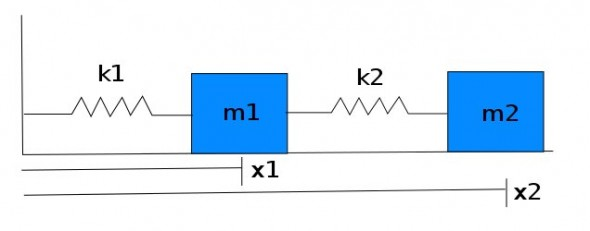
\includegraphics[width=0.8\columnwidth]{mass-spring.jpg}
%\end{figure}
%
%\par \textbf{Solution} We can use Newton's second law and Hooke's law to derive the following equations. Note that when deriving the spring force on a mass when the ends of the spring are each attached to a mass, we calculate $\Delta x$ as 
%\[ \Delta x = (\text{mass being acted on}) - (\text{mass on other end})\]
%This is how we derive the equation for the second term in the first equation, and the entirety of the second equation. 
%\begin{align*}
%m_1x_1'' &= -k_1x_1 -k_2(x_1 - x_2) \\
%m_2x_2'' &= -k_2 (x_2 - x_1) 
%\end{align*}
%\par A much craftier (and ultimately easier) way to derive the system is through the \textit{principle of least action}. This is one of the most important methods in all of physics and engineering, but is also rarely taught at the undergraduate level. To begin, we first calculate the Lagrangian of the system 
%\[ \mathcal{L} = T - U \]
%where $T$ represents the total kinetic energy of the system, and $U$ represents the potential energy. Note that for physical systems, this will always be negative, which is a consequence of conservation of energy. You can think of the Lagrangian as the ``leftover'' energy in the system. Indeed, this is very closely related to the Lagrangian we encountered in constrained optimization in CME 100 --- in optimization, the optimal solution is the one which requires the least energy. 
%\par After calculating the Lagrangian, we can form the \textit{Euler-Lagrange equations} for $i$ variables in our system through the relation:
%\[ \frac{\partial \mathcal{L}(t,x,x') }{\partial x_i} - \frac{d}{dt} \left( \frac{\partial  \mathcal{L}(t,x,x') }{\partial x'_i}\right) = 0\]
%This equation is a bit ungainly since we are taking derivatives with respect to both the state variables $x$ and $x'$ \textit{treating them as separate variables} (i.e. chain rule does not apply), as well as our independent variable $t$. However, as we will see in this example, doing this is actually quite straight-forward. We can take these derivatives for all $i$ variables, which will give us the differential equations for the system.
%
%\par Lets now derive the differential equations for this system using the Euler-Lagrange equations. First derive the Lagrangian. Here, we will have kinetic energy from the masses, as well as potential energy stored in the springs. So, the Lagrangian is:
%\[ \mathcal{L} = \underbrace{\frac{1}{2} m_1 x_1'^2}_{\text{K.E. from mass 1}} + \underbrace{\frac{1}{2} m_2 x_2'^2}_{\text{K.E. from mass 2}} - \underbrace{\frac{1}{2} k_1 x_1^2}_{\text{P.E. from spring 1}} - \underbrace{\frac{1}{2} k_2 (x_2 - x_1)^2}_{\text{P.E. from spring 2}} \]
%
%Now, form the Euler-Lagrange equations:
%\begin{align*}
%0 &= \frac{\partial \mathcal{L}(t,x,x') }{\partial x_1} - \frac{d}{dt} \left( \frac{\partial  \mathcal{L}(t,x,x') }{\partial x'_1}\right) \\
%&= -k_1x_1 + k_1(x_2 - x_1) - \frac{d}{dt}\left( m_1 x_1' \right) \\
%m_1 x_1'' &= -k_1x_1 - k_1(x_1 - x_2) \\
%0 &= \frac{\partial \mathcal{L}(t,x,x') }{\partial x_2} - \frac{d}{dt} \left( \frac{\partial  \mathcal{L}(t,x,x') }{\partial x'_2}\right) \\
%&= -k_1(x_2 - x_1) - \frac{d}{dt} \left( m_2 x_2' \right)\\
%m_2 x_2'' &= -k_1(x_2 - x_1)
%\end{align*}
%Do these look familiar?
%\par \textbf{Remark:} Even if you do not plan to use this on the exam, please take some time to read up on the Principle of Least Action. Richard Feynman gives an excellent exposition in his lectures on physics, and there are plenty of other resources online as well. This is one of the most important ideas in all of science and engineering---indeed, it is one of the only physical laws (if not the only law) that holds at all scales---and allows us to link the otherwise disparate realms of optimization theory and physical systems. 

\clearpage
\item \textbf{Higher Order ODEs and MATLAB}
\begin{enumerate}
\item A system of couple pendulums could be modeled by the following system of equations: 
\begin{gather*}
\theta_a'' + \theta_b'' + \frac{g}{\ell}\theta_a + \frac{K}{M}(\theta_a - \theta_b) = 0 \tag{1}\\
\theta_a'' + 2 \theta_b'' + \frac{g}{\ell}\theta_b + \frac{K}{M}(\theta_b - \theta_a) = 0 \tag{2}
\end{gather*}


\begin{enumerate}[label=(\roman*)]
\item Rewrite this as a coupled system of first-order ODEs.
%\par \textbf{Solution:} We first need to introduce our ``dummy variables'' and define our state vector for the system. When converting a higher order system into a first order system, this is the most important and often trickiest part. 
%\par Every variable in the system (in this case, $\theta_a$ and $\theta_b$) has \textit{as many states as its highest derivative}. That is, if the second derivative exists in the system, we need to put that variable and its first derivative in the state vector. (You can think of this as each derivative creating a degree of freedom in the system, so we need to solve for both the function and its lower derivatives when finding a solution to the ODE in order to eliminate these extra degrees of freedom and have a unique solution.)
%\par The given system is second order in both $\theta_a$ and $\theta_b$, so our state vector must include $\theta_a$, $\theta_a'$, $\theta_b$, and $\theta_b'$. So, let $v_1 = \theta_a$, $v_2 = \theta_b$, $v_3 = \theta_a'$, and $v_4 = \theta_b'$ for our state vector $\vec v$. 
%\par Substitute these into the system, and algebraically manipulate the system to find $\vec v' = f(\vec v)$:
%\begin{align*}
%0 &= v_3' + v_4' + \frac{g}{\ell}v_1 + \frac{K}{M}(v_1 - v_2) \tag{1} \\
%0 &= v_3' + 2 v_4' + \frac{g}{\ell}v_2 + \frac{K}{M}(v_2 - v_1) \tag{2}
%\intertext{$(2) - (1)$:}
%0 &= v_4'+ \frac{g}{\ell}(v_2 - v_1) + 2\frac{K}{M}(v_2 - v_1) \\
%v_4' &= \frac{g}{\ell}(v_1 - v_2) + 2\frac{K}{M}(v_1 - v_2)  \\
%\intertext{$(2) - 2\times (1)$:}
%0 &= -v_3' + \frac{g}{\ell} (v_2 - 2v_1) + 3 \frac{K}{M}(v_2 - v_1) \\
%v_3' &= \frac{g}{\ell} (v_2 - 2v_1) + 3 \frac{K}{M}(v_2 - v_1) \\
%\intertext{Then the trivial relations:}
%v_1' &= v_3\\
%v_2'&= v_4
%\intertext{Combining these into matrix form:}
%\left[ \begin{array}{c} v_1' \\ v_2' \\ v_3' \\ v_4' \end{array} \right] &= \left[ \begin{array}{cccc} 0 & 0 & 1 & 0 \\ 0 & 0 & 0 & 1 \\ -2\frac{g}{\ell} - 3\frac{K}{M} & \frac{g}{\ell} + 3\frac{K}{M} & 0 & 0 \\ \frac{g}{\ell} + 2\frac{K}{M} & -\frac{g}{\ell} - 2\frac{K}{M} & 0 & 0 \end{array} \right] \left[ \begin{array}{c} v_1 \\ v_2 \\v_3 \\v_4 \end{array} \right] \quad\blacksquare 
%\end{align*}


\item Write a MATLAB function to evaluate the derivative such that the system could be solved with \texttt{ode45()}. Pass in $g$, $\ell$, $K$, and $M$ as parameters.
%\par \textbf{Solution:} Since the ODE is linear and we've already put it into matrix form, this function is very easy to write. The only thing we must keep in mind is that \texttt{ode45()} requires that the derivative be output as a column vector. However, because we have formulated this as a matrix mapping a column vector to another column vector, this requirement is already satisfied. The code below will be compatible with \texttt{ode45()}:
%
%\begin{lstlisting}
%function yp = derivative(x,y, g, l, K, M)
%	A = [0, 0, 1, 0; ...
%		0, 0, 0, 1; ...
%		-2*g / l - 3*K / M, g / l + 3 * K / M, 0, 0;...
%	 	g / l + 2*K / M, -g / l - 2 * K / M, 0, 0];
%	yp = A*y;
%end
%
%\end{lstlisting}

Note that there are many correct ways to write this function, this is just one example. 

\item Write a script to call \texttt{ode45()} to solve this ODE over the domain $0 \leq t \leq 10$ with initial conditions:
\[ \theta_a = \pi, \; \theta_b = 0, \; \theta_a'(0) = 0, \; \theta_b'(0) = 0 \]
Include code to plot the solution for $\theta_b$ as a function of $t$. Use the values $g = \ell = K = M = 1$ and pass these in as parameters to your \texttt{yp()} function. 
%\par \textbf{Solution:}
%One example of a script that would do this:
%\begin{lstlisting}
%clear all; close all
%
%g = 1; l = 1; K = 1; M = 1;
%[t, y] = ode45(@(t,y) yp(t,y, g, l, K M), [0, 10], [pi, 0, 0, 0])
%plot(t, y(:,2))
%\end{lstlisting}

\end{enumerate}


\item For the following initial value problem
\[ y'' + x^2y' + y = 1,\quad y(0) = 1, \quad y'(0) = 1 \]
write a piece of MATLAB code to numerically solve the system using Backward Euler method. Use step size $h = 0.1$, solve over interval $x \in [0,1]$, and include code to plot your solution. 

%\par\textbf{Solution:}
%We first must rewrite this as a system of first-order ODEs. Introduce ``dummy variables'' $v_1 = y$ and $v_2 = y'$. The ODE then becomes:
%\[ v_2' + x^2 v_2 + v_1 = 1 \]
%We can then rewrite this as a first order (nonlinear) system for $\vec v' = f(\vec v)$:
%\begin{align*}
%v_1' &= v_2\\
%v_2' &= 1 - v_1 - x^2 v_2
%\end{align*}
%
%Now, recall the equation for the backward Euler method:
%\[ \vec y_{i+1} = \vec y_i + h \vec y'(x_{i+1}, \vec y_{i+1}) \]
%We can plug our expression for $\vec v'$ into this equation then algebraically solve for $\vec v_{i+1}$ to find the final expressions:
%
%\begin{align*}
%\vec v_{i+1} &= \vec v_i + h \left[ \begin{array}{c} v_{2,i+1} \\ 1 - v_{1,i+1} - x_{i+1}^2 v_{2,i+1} \end{array} \right]\\
%\left[ \begin{array}{c} v_{1,i+1} \\ v_{2,i+1} \end{array} \right] &= \left[ \begin{array}{c} v_{1,i} \\ v_{2,i} \end{array} \right]+ h \left[ \begin{array}{c} v_{2,i+1} \\ 1 - v_{1,i+1} - x_{i+1}^2 v_{2,i+1} \end{array} \right]
%\intertext{Plugging the first equation into the second:}
%v_{2,i+1} &= v_{2,i} + h\left (1 - (v_{1,i} + hv_{2,i+1}) - x_{i+1}^2 v_{2,i+1}\right) \\
%&=  v_{2,i} +  h - hv_{1,i} - h^2 v_{2,i+1} - hx_{i+1}^2 v_{2,i+1} \\
%v_{2,i+1}  + h^2 v_{2,i+1} + hx_{i+1}^2 v_{2,i+1} &= v_{2,i} + h - hv_{1,i} \\
%v_{2,i+1} &= \frac{1}{1 + h^2 + hx_{i+1}^2} \left( v_{2,i} + h - hv_{1,i} \right)
%\intertext{We can then plug this into the equation for $v_{1,i+1}$ to find our final system:}
%\left[ \begin{array}{c} v_{1,i+1} \\ v_{2,i+1} \end{array} \right] &= \left[ \begin{array}{c} v_{1,i} +  \frac{h}{1 + h^2 + hx_{i+1}^2} \left( v_{2,i} + h - hv_{1,i} \right)\\ \frac{1}{1 + h^2 + hx_{i+1}^2} \left( v_{2,i} + h - hv_{1,i} \right)\end{array} \right]
%\end{align*}
%
%Now that we have our system solved for $\vec v_{i+1}$ in closed form, we can easily implement the numerical solution in MATLAB:
%
%\begin{lstlisting} 
%h = 0.1;
%x = 0; 
%xmax = 10;
%v(1,1) = 1;
%v(2,1) = 1;
%i = 1;
%
%while x < xmax
%	x(i+1) = x(i) + h;
%	v(1,i+1) = v(1,i) + (h/(1 + h^2 + h(x(i+1)^2)))*(v(2,i) + h - h*v(1,i));
%	v(2,i+1) = (1/(1 + h^2 + h(x(i+1)^2)))*(v(2,i) + h - h*v(1,i));
%	i = i+1;
%end
%
%plot(x,v(1,:))
%
%\end{lstlisting}
\end{enumerate}

\end{enumerate}

%----------------------------------------------------------------------------------------

\end{document}